\section{Análisis}

\subsection{Contexto}

\subsubsection{Descripción General}

Este proyecto busca, mostrar los museos de manera más interactiva utilizando RA y código QR, permitiendo a sus usuarios no solo acceder a las piezas expuestas en los museos, sino que también visualizar el interior de los museos y poder interactuar con dichas piezas que historicas.


\subsubsection{Descripción de Clientes y Usuarios:}

Esta aplicación apunta dos tipos de usuarios principalmente, el primero 1 más relevante dentro del objetivo entregar la cultura es a estudiantes de finales de 2do ciclo (enseñanza básica) y estudiantes de 3er ciclo (enseñanza media) es decir de 6to básico a 4to medio, este grupo esta compuestos por personas de alrededor de 11 a 19 años de edad y que están en un periodo de formación educacional, además consideramos como segundo grupo clave de usuarios a personas que ya estén interesadas en museos, cualquiera sea su edad, y por sobretodo a las interesadas en las tecnologías realidad aumentada.

En base al grupo principal de usuarios se destaca que los mayores interesados en educarlos son sus padres o tutores además de la institución educativa a la cual pertenecen y su docentes, es por esto que como principal generador de demanda estarán estas instituciones, y como principal cliente se acudirá al ministerio de educación y entes preocupados por la educación de los jóvenes chilenos.

Como alianza extra se abrirá suscripción a museos a que estén interesados en aparecer dentro de esta aplicación, esto les dará una nueva canal de comunicación con las personas interesadas en ellos, además de la obtención de información por medio de nuestra aplicación.


\subsection{Especificación de Requerimientos}

\subsubsection{Funciones del Sistema}

\begin{longtable}{|c|p{10cm}|c|}
\hline 
Ref\# & Función & Categoría (E/O/S) \\ 
\hline 
1.1 & Iniciar juego al presionar en el medio de la pantalla con la app abierta. & E \\ 
\hline 
1.2 & Mostrar título del juego & E \\ 
\hline 
1.3 & Escanear código & E \\ 
\hline 
1.4 & Mostrar museo correspondiente al código Escaneado & E \\ 
\hline 
2.1 & Visualizar pieza en 3d situada en el museo & E \\ 
\hline 
2.2 & Obtener modelo de las piezas & O \\ 
\hline 
2.3 & Interactuar con la pieza & E \\ 
\hline 
2.4 & Visualizar pieza en 3d en el panel de información & E \\ 
\hline 
2.5 & Desplegar visualizador de pieza & E \\ 
\hline 
2.6 & Desplegar ventana de manipulación de pieza & E \\ 
\hline 
2.7 & Obtener información de las piezas & O \\ 
\hline 
2.8 & Mostrar información de las piezas & E \\ 
\hline 
3.1 & Activar/Desactivar menú desplegable de opciones y características & E \\ 
\hline 
3.2 & Silenciar aplicación & S \\ 
\hline 
3.3 & Redireccionar a pagina de la aplicación & S \\ 
\hline 
3.4 & Mostrar Guia/Tutorial de uso básico de la app & E \\ 
\hline 
3.5 & Tutorial de manejo de pieza & E \\ 
\hline 
4.1 & Construir mensaje al compartir en RRSS & O \\ 
\hline 
4.2 & Obtener información de la pieza para compartir en RRSS & O \\ 
\hline 
4.3 & 
Desplegar menú para compartir en RRSS
 & E \\ 
\hline 
4.4 & Obtener información del museo para compartir en RRSS & O \\ 
\hline 
5.1 & Desplegar menú de museos & E \\ 
\hline 
5.2 & Mostrar museos visitados y no visitados & E \\ 
\hline 
5.3 & Obtener información de museos & O \\ 
\hline 
5.4 & Desplazarse entre los museos & E \\ 
\hline 
5.5 & Cerrar ventana de museos & E \\ 
\hline 
5.6 & Descargar QR del museo & O \\ 
\hline 
5.7 & Buscador de museo & E \\ 
\hline 
5.8 & Zoom Museo & E \\ 
\hline 
5.9 & Desplazarse por el museo virtual & E \\ 
\hline 
5.1.1 & Mostrar la descarga del QR del museo & E \\ 
\hline 
5.1.2 & Mostrar información de los museos & E \\ 
\hline 
6.1 & Desplegar menu de piezas & E \\ 
\hline 
6.2 & Retroceder al menú de museos & E \\ 
\hline 
6.3 & Desplazarse entre las piezas & E \\ 
\hline 
6.4 & Mostrar piezas obtenidas y no descubiertas & E \\ 
\hline 
6.5 & Obtener información de piezas & O \\ 
\hline 
6.6 & Cerrar ventana de piezas & E \\ 
\hline 
6.7 & Zoom Pieza & E \\ 
\hline 
6.8 & Rotación pieza & E \\ 
\hline 
7.1 & Desplegar menu para visualizar logros & E \\ 
\hline 
7.2 & Cerrar ventana de logros & E \\ 
\hline 
7.3 & Obtener información de logros & O \\ 
\hline 
7.4 & Mostrar logros obtenidos y no completados & E \\ 
\hline 
7.5 & Desplazarse entre los logros & E \\ 
\hline 
7.6 & Visualizar nuevo logro & E  \\ 
\hline 
\caption{Tabla de Funciones de Sistema}
\label{tab18}\\
\end{longtable}


\subsubsection{Atributos del Sistema}

\begin{longtable}{|c|p{3.5cm}|p{10cm}|}
\hline 
Ref\# & Atributo & Detalle y limitación \\ 
\hline 
AT1.1 & Tiempo de respuesta del escaneo & Menor a 1.5 segundos para informar al usuario que se detectó el código y menor a 7 para mostrar el contenido final.  \\ 
\hline 
AT1.2 & Uso en móvil gama media & XXXX  \\ 
\hline
AT1.3 & Interfaz implementada con iconos & Cualquier usuario debe ser capaz de orientarse en la aplicación sin importar su edad (dentro de las estipuladas en los grupos usuarios) o idioma (que saber español o inglés no sea un requerimiento para ocupar la app).  \\ 
\hline
AT1.4 & Información presentada de manera simple y legible & Tanto la información de las piezas como la de los museos debe ser presentada en un formato que no abrume al usuario, debe ser digerible y fácil de leer.  \\ 
\hline
AT1.5 & Tutoriales simples y autoexplicativo & Cada nuevo sistema dentro de la aplicación debe ser enseñado a través de un tutorial que muestre una imagen de ejemplo de lo que se está explicando y un texto que describa la situación como mínimo.	\\ 
\hline
AT1.6 & Mantener al usuario interesado, evitar que se frustre & Las piezas a encontrar  siempre deben tener un leve feedback para que el jugador note su presencia, además si el usuario pasa más de 40 segundos en una habitación con una pieza esta debe mostrarse de manera aún más notable, si esto supera los 90 segundos se debe mostrar de forma evidente su ubicación.  \\ 
\hline
AT1.7 & XXXX & XXXX  \\ 
\hline
\caption{Tabla de Atributos del Sistema}
\label{tab19}\\
\end{longtable}

\subsubsection{Atributos por Función}

\begin{longtable}{|c|p{4.7cm}|p{1.8cm}|p{4.7cm}|p{1.8cm}|}
\hline 
Ref\# & Función & Categoría (E/O/S) & Atributo & Categoría (E/R/D)\\ 
\hline 
R1.1 & Escaneo codigo & E & Tiempo de respuesta del escaneo & R \\ 
\hline 
R1.2 & Visualizar pieza 3D & E & Uso en móvil gama media & E \\ 
\hline
R1.3 & Obtener información de las piezas & E & Información presentada de manera simple y legible & R \\ 
\hline
R1.4 & Mostrar guia/tutorial de uso básico de app & E & Tutoriales simples y autoexplicativo & D \\ 
\hline
\caption{Tabla de Atributos por Función}
\label{tab20}\\
\end{longtable}

\newpage
\subsection{Actores}

\subsubsection{Clientes}
Se establece como cliente, al organismo gubernamental que el cual está encargado de la historia y cultura patrimonial. Además de organismos privados quienes manejan museos abiertos a todo público quienes quieren fomentar el conocimiento cultural.

\begin{enumerate}
	\item Gobierno de chile / Ministerio de la cultura.
	\item Museos interesados en aparecer en la app.
\end{enumerate}

\subsubsection{Usuarios}
Se establece como usuario a toda persona que se encuentre actualmente cursando su segundo ciclo de enseñanza escolar correspondiente a finales de enseñanza básica y enseñanza media.

\begin{enumerate}
	\item Estudiantes enseñanza media.
	\item Aficionados de museos.

\end{enumerate}

\subsection{Casos de Uso}

%%%%%%% CASO-1 %%%%%%%%%%%%%%%%
\newpage
\subsubsection{Primera interacción con la aplicación dentro de la sala de clases}

{\textbf {Resumen:}}
El usuario (alumno enseñanza media) luego de que su profesor le hiciera entrega de una guía con la imagen QR de uno de los museos, descarga la aplicación indicada en esta, al terminar de descargar la app, la inicia, activa la cámara y apunta a la imagen con ella, al hacer esto el usuario visualiza sobre la imagen como se dibuja la habitación de un museo y ve en las indicaciones en pantalla, este se da cuenta de que puede explorar en la habitación para encontrar las piezas que esté muestra las cuales están escondidas dentro de este entorno. Además prueba las diferentes acciones para desplazarse por el museo. Luego al encontrar una pieza el usuario presiona sobre ella y descubre que ha encontrado un objeto, el cual es añadido a su colección de piezas, el usuario entusiasmado voltea a mostrarle a sus compañeros el descubrimiento.

{\textbf {Actores:}}
Alumno enseñanza media, Profesor.

{\textbf {Propósito:}}
Introducir al alumno el aprendizaje del museo local en cuestión, el cual se encuentra presente en la guía entregada por el profesor.

{\textbf {Tipo:}}
Primario.

{\textbf {Referencias cruzadas:}}
R 1.1, R 1.2, R 1.3, R 2.1, R 2.2, R 2.7, R 3.4, R 5.9.

\paragraph{Caso de Uso Esencial}

\begin{longtable}{|p{5cm}|p{8cm}|}
\hline 
Acción actores & Respuesta del sistema \\ 
\hline 
El profesor entrega al alumno el código QR & --- \\ 
\hline
El alumnos descarga la aplicación & Se muestran las indicaciones del uso necesario de la cámara \\ 
\hline 
El alumno enciende la cámara  & Se muestran las indicaciones de cómo interactúa con el código QR \\ 
\hline
El alumno apunta el código QR con su cámara & La aplicación detecta el código y carga un modelo 3d correspondiente al museo ligado a ese código.
Se le presentan las instrucciones de desplazamiento en el museo y se le informa que puede encontrar las piezas, del museo si las busca.
 \\ 
\hline
El alumno prueba las instrucciones de desplazamiento. & La aplicación cambia el escenario mostrado de acuerdo a las acciones hechas por el usuario. \\ 
\hline
El jugador ve una pieza y la presiona. & El sistema muestra una animación que confirma el haber encontrado la pieza y muestra una panel con información más detallada de esta \\ 
\hline
El alumno se voltea a mostrar su descubrimiento a su compañero. & --- \\ 
\hline
\end{longtable}

\paragraph{Diagrama de Caso de Uso}

\begin{figure}[H]
\centerline{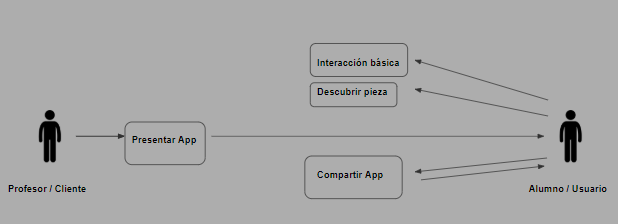
\includegraphics[width=15cm]{imgs/CasoUso_1.PNG}}
\caption{Caso-1}
\label{fig}
\end{figure}

\paragraph{Modelo Conceptual}

\begin{figure}[H]
\centerline{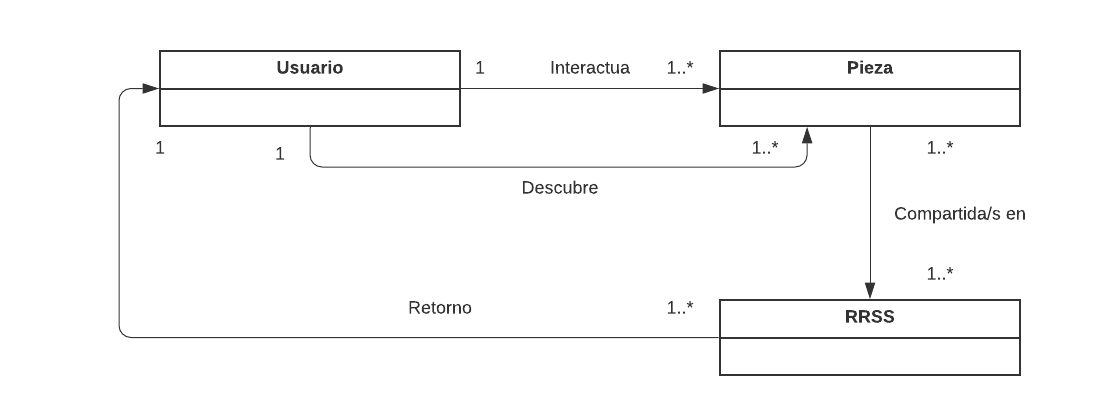
\includegraphics[width=15cm]{imgs/ModeloConceptualCaso_1_3.png}}
\caption{Caso-1}
\label{fig}
\end{figure}

\paragraph{Diagrama de Secuencia o Colaboración}

\begin{figure}[H]
\centerline{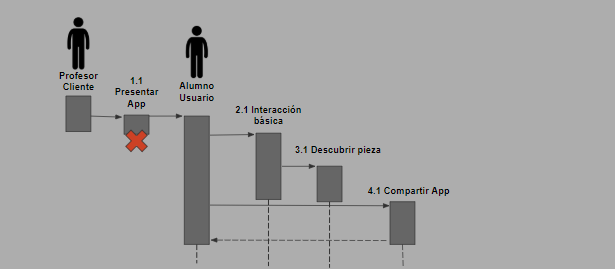
\includegraphics[width=15cm]{imgs/CasoUso_1_2.PNG}}
\caption{Caso-1}
\label{fig}
\end{figure}

\subsubsection{Priorización}
{\textbf {Tipo:}}
Primario.

%%%%%%% CASO-2 %%%%%%%%%%%%%%%%
\newpage
\subsubsection{Uso de la aplicacion por personas sin español como idioma nativo}

{\textbf {Resumen:}}
Un usuario extranjero llega a un museo local es su ruta de turismo, al ver un cartel de la App en el museo la descarga, luego en su alojamiento decide probar la aplicación, al abrirla este se encuentra con una serie de imágenes que le muestran cómo ocupar la aplicación, estas imágenes están acompañadas de un texto en español pero el logra sin ningún problema a ocupar la aplicación.

{\textbf {Actores:}}
Usuario de nacionalidad extranjera (no chileno), Museo/Publicidad.

{\textbf {Propósito:}}
Lograr que una persona que no maneja el lenguaje nacional logre interactuar con la aplicación sin problemas, adems de demostrar su uso de manera internacional.

{\textbf {Referencias cruzadas:}}
R 1.1, R 1.2, R1.3, R3.4, R3.5

\paragraph{Caso de Uso Esencial}

\begin{longtable}{|p{5cm}|p{8cm}|}
\hline 
Acción actores & Respuesta del sistema \\ 
\hline 
XXXX & XXXX \\ 
\hline 
\end{longtable}

\paragraph{Diagrama de Caso de Uso}

\begin{figure}[H]
\centerline{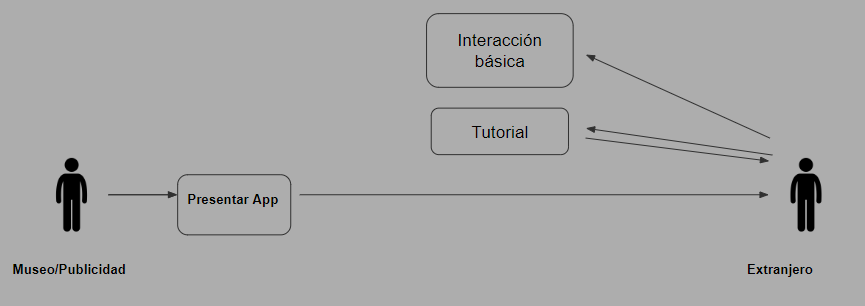
\includegraphics[width=15cm]{imgs/CasoUso_2.PNG}}
\caption{Caso-1}
\label{fig}
\end{figure}

\subsubsection{Modelo Conceptual}

\begin{figure}[H]
\centerline{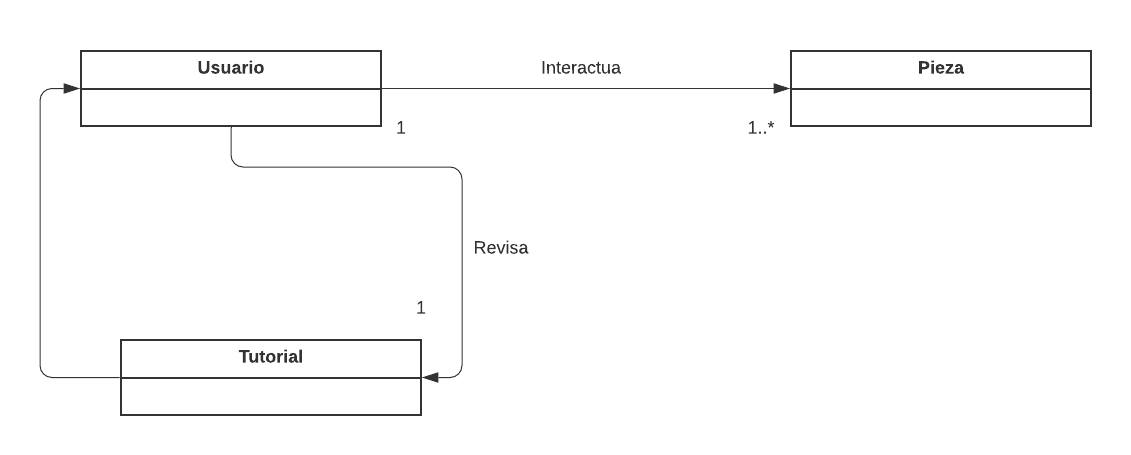
\includegraphics[width=15cm]{imgs/ModeloConceptualCaso_2_3.png}}
\caption{Caso-1}
\label{fig}
\end{figure}

\paragraph{Diagrama de Secuencia o Colaboración}

\begin{figure}[H]
\centerline{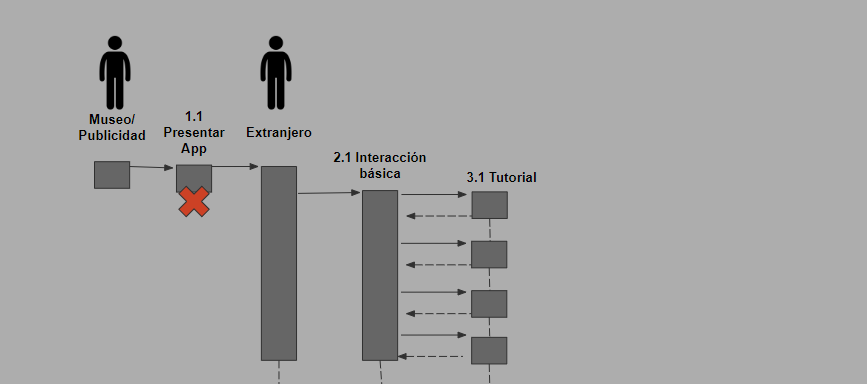
\includegraphics[width=15cm]{imgs/CasoUso_2_2.PNG}}
\caption{Caso-1}
\label{fig}
\end{figure}

\paragraph{Priorización}
{\textbf {Tipo:}}
Relevante.

%%%%%%% CASO-3 %%%%%%%%%%%%%%%%
\newpage
\subsubsection{situacion de pompetitividad entre jovenes}

{\textbf {Resumen:}}
Dos estudiantes están compartiendo y mostrando el uno al otro las piezas que han encontrado en sus museos virtuales, cuando alguno de ellos tiene una pieza que el otro no este le explica en qué parte del museo virtual está y generan una conversación en base a la pieza historica.

{\textbf {Actores:}}
Estudiante-1, Eestudiante-2.

{\textbf {Propósito:}}
Mostrar el uso social de la aplicación dentro del colegio y usar la competitividad como herramienta de aprendizaje.

{\textbf {Referencias cruzadas:}}
R1.1,R1.2, R6.1, R6.2, R6.3, R6.4, R6.6

\paragraph{Caso de Uso Esencial}

\begin{longtable}{|p{5cm}|p{8cm}|}
\hline 
Acción actores & Respuesta del sistema \\ 
\hline 
Los estudiantes navegan por los menús de piezas dentro de la aplicación. & La aplicación va mostrando un listado de piezas marcando las que tienen descubiertas.
estas piezas están separadas por temática y numeradas.
 \\ 
\hline 
Los estudiantes comparan cada casilla, entre ambos dispositivos. & --- \\
\hline 
Al encontrar casillas vacías en los dispositivos del otro le comenta cual es y cómo encontrarla.  & --- \\
\hline 
\end{longtable}

\paragraph{Diagrama de Caso de Uso}

\begin{figure}[H]
\centerline{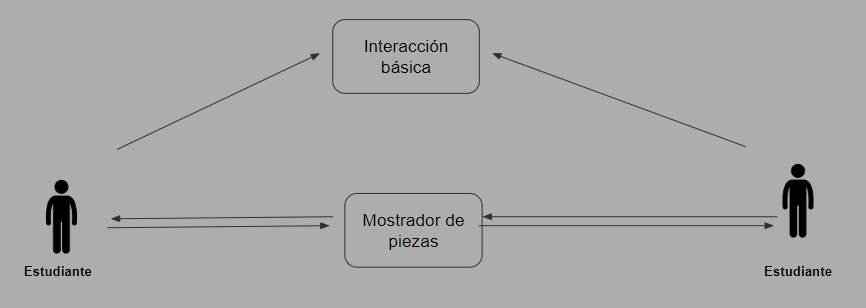
\includegraphics[width=15cm]{imgs/CasoUso_3.PNG}}
\caption{Diagrama Caso 3}
\label{fig_3_1}
\end{figure}

\paragraph{Modelo Conceptual}

\begin{figure}[H]
\centerline{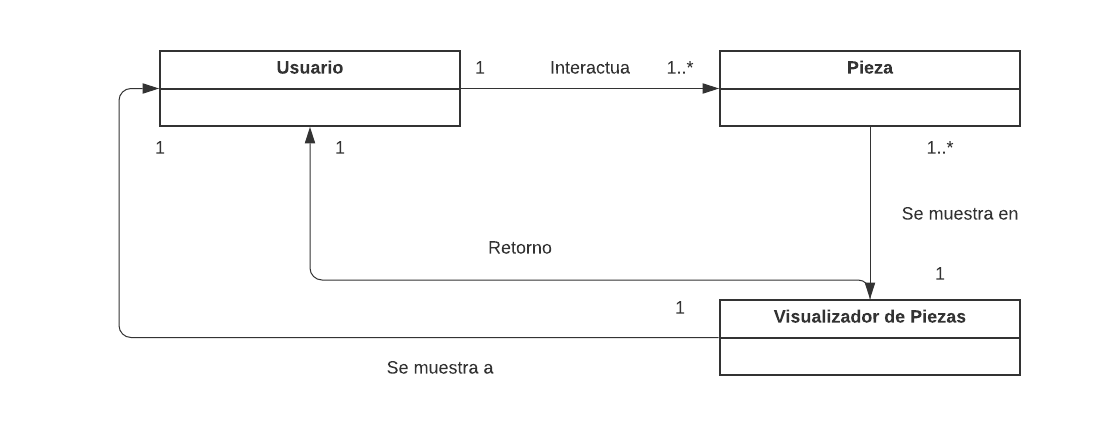
\includegraphics[width=15cm]{imgs/ModeloConceptualCaso_3_3.png}}
\caption{Modelo Conceptual Caso 3}
\label{fig_3_2}
\end{figure}


\paragraph{Diagrama de Secuencia o Colaboración}

\begin{figure}[H]
\centerline{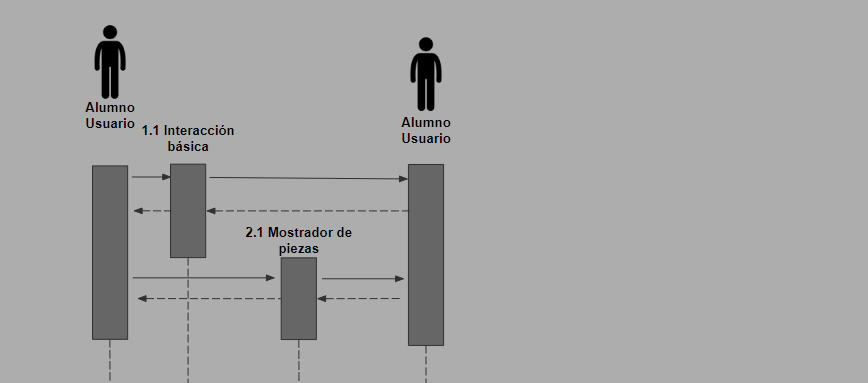
\includegraphics[width=15cm]{imgs/CasoUso_3_2.PNG}}
\caption{Diagrama de Secuencia Caso 3}
\label{fig_3_3}
\end{figure}

\paragraph{Priorización}
{\textbf {Tipo:}}
Relevante.

%%%%%%% CASO-4 %%%%%%%%%%%%%%%%
\newpage
\subsubsection{Presentacion de estudiente para su curso}

{\textbf {Resumen:}}
Un alumno de enseñanza media tiene que hacer una presentación sobre un tema histórico local, el recuerda que hay informacion de esto en el museo pero no puede ir por cuarentena (COVID), a su vez recuerda que en la aplicación “museo en casa” tiene esa pieza en su colección, días después el estudiante presenta sin problemas ya que pudo obtener la información necesaria para esta desde la información entregada por la aplicación.

{\textbf {Actores:}}
Estudiante.

{\textbf {Propósito:}}
Mostrar usos prácticos de la aplicación que no tengan una relación directa con su parte lúdica.

{\textbf {Referencias cruzadas:}}
R1.1, R1.2, R2.7,R2.8, R5.3, R6.1, R6.5

\paragraph{Caso de Uso Esencial}

\begin{longtable}{|p{5cm}|p{8cm}|}
\hline 
Acción actores & Respuesta del sistema \\ 
\hline 
El alumno abre la aplicación y entra al menu de piezas & La aplicación muestra un listado de las piezas. \\ 
\hline
El alumno ocupa el buscador de pieza para encontrar la que necesita en su presentación. & La aplicación solo muestra la información relacionada a lo ingresado por el usuario. \\ 
\hline 
El jugador encuentra, la pieza que busca y la clickea. & El sistema abre un panel con la información de la pieza independiente si esta la tiene en su colección pero no las opciones lúdicas. \\ 
\hline 
El usuario utiliza la aplicación como fuente de datos para su presentación y no se preocupa de no disponer de las opciones lúdicas ya que no son necesarias. & --- \\ 
\hline 
\end{longtable}

\paragraph{Diagrama de Caso de Uso}

\begin{figure}[H]
\centerline{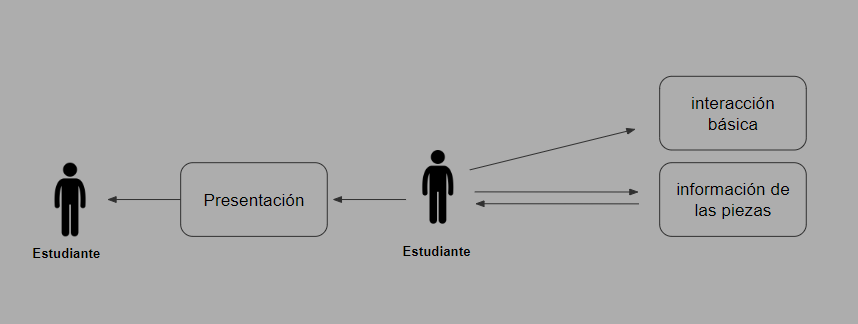
\includegraphics[width=15cm]{imgs/CasoUso_4.PNG}}
\caption{Diagrama Caso 4}
\label{fig_4_1}
\end{figure}

\paragraph{Modelo Conceptual}

\begin{figure}[H]
\centerline{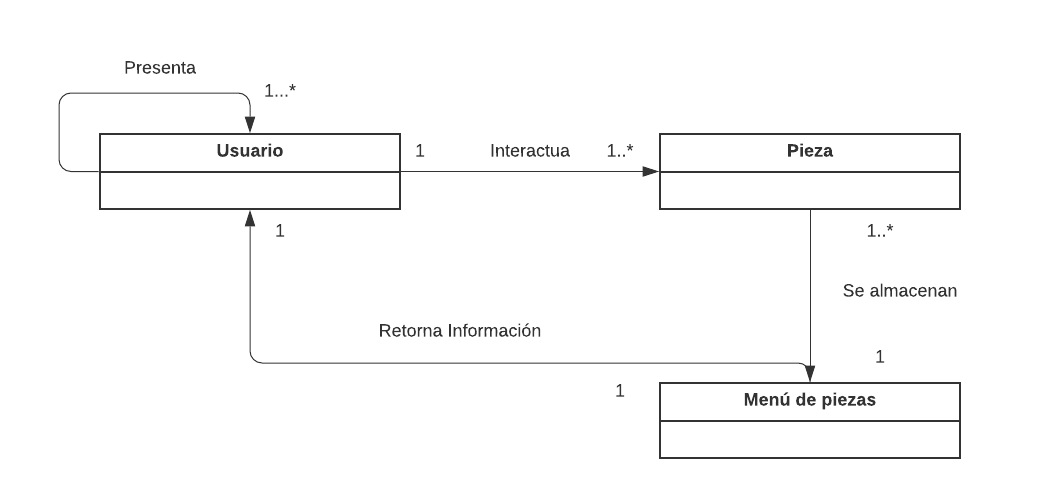
\includegraphics[width=15cm]{imgs/ModeloConceptualCaso_4_3.png}}
\caption{Modelo Conceptual Caso 4}
\label{fig_4_2}
\end{figure}


\paragraph{Diagrama de Secuencia o Colaboración}

\begin{figure}[H]
\centerline{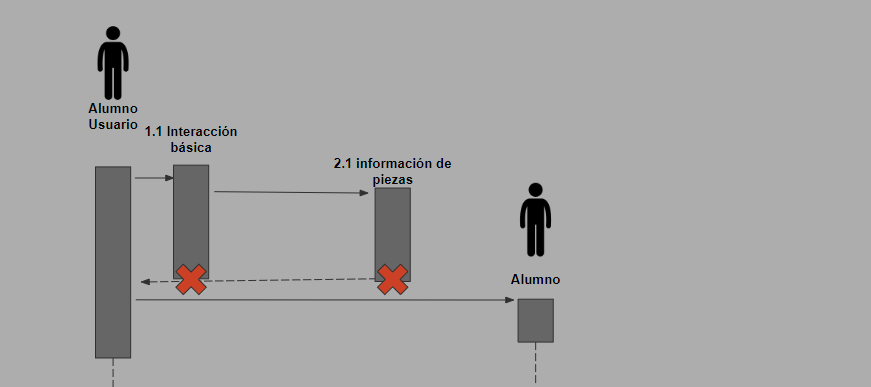
\includegraphics[width=15cm]{imgs/CasoUso_4_2.PNG}}
\caption{Diagrama de Secuencia Caso 4}
\label{fig_4_3}
\end{figure}

\paragraph{Priorización}
{\textbf {Tipo:}}
Deseable.

%%%%%%% CASO-5 %%%%%%%%%%%%%%%%
\newpage
\subsubsection{Excursión de grupo escolar}

{\textbf {Resumen:}}
Un profesor decide llevar a su grupo de estudiantes a una excursión para el museo, algunos estudiantes no se ven entusiasmado con la idea así que el profesor los desafía a encontrar las piezas del museo en la app “Museo en casa”. Durante el trayecto de la excursión los alumnos aprovechan de revisar la información del museo y de las piezas en el para que al llegar al museo ya sepan que es lo que tienen que buscar.

{\textbf {Actores:}}
Estudiantes (plural), Profesor.

{\textbf {Propósito:}}
Apoyo didáctico y lúdico para actividades que son llevadas por instituciones educativas durante el periodo normal de clases.

{\textbf {Referencias cruzadas:}}
R1.1, R1.2, R4.4, R5.2, R5.3, R5.4, R5.5, R5.7, R5.1.2

\paragraph{Caso de Uso Esencial}

\begin{longtable}{|p{5cm}|p{8cm}|}
\hline 
Acción actores & Respuesta del sistema \\ 
\hline 
XXXX & XXXX \\ 
\hline 
\end{longtable}

\paragraph{Diagrama de Caso de Uso}

\begin{figure}[H]
\centerline{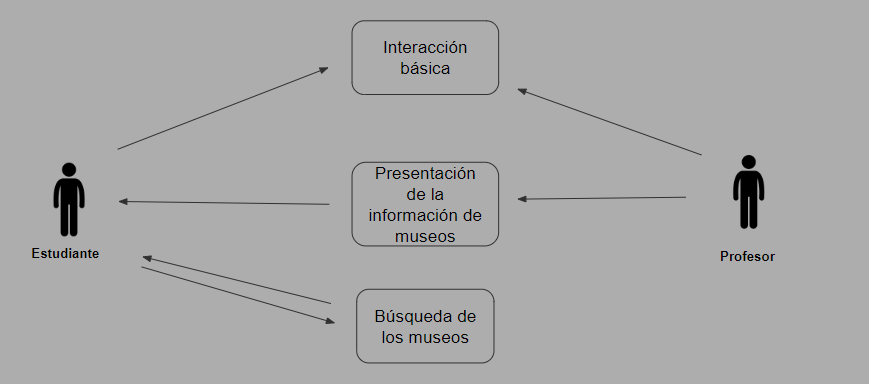
\includegraphics[width=15cm]{imgs/CasoUso_5.PNG}}
\caption{Caso-1}
\label{fig}
\end{figure}

\paragraph{Modelo Conceptual}

\begin{figure}[H]
\centerline{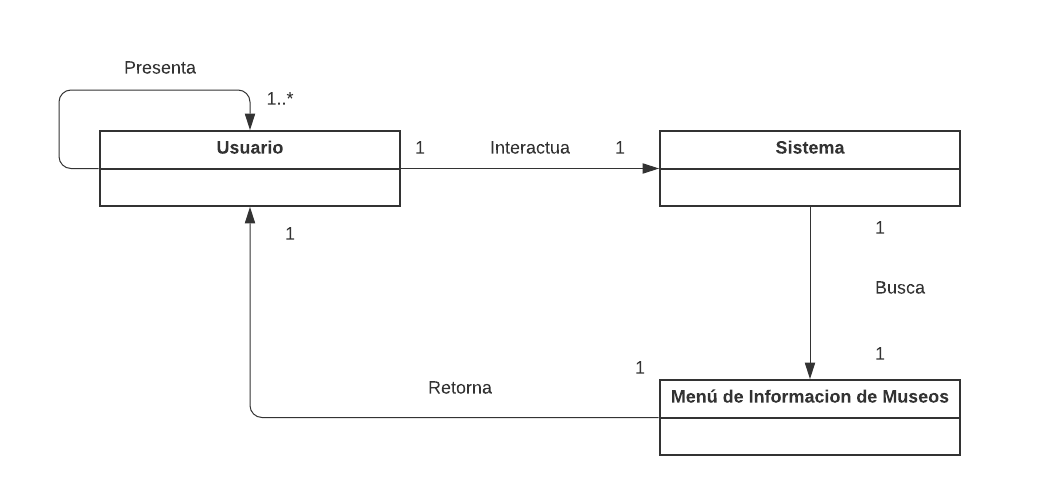
\includegraphics[width=15cm]{imgs/ModeloConceptualCaso_5_3.png}}
\caption{Caso-1}
\label{fig}
\end{figure}


\paragraph{Diagrama de Secuencia o Colaboración}

\begin{figure}[H]
\centerline{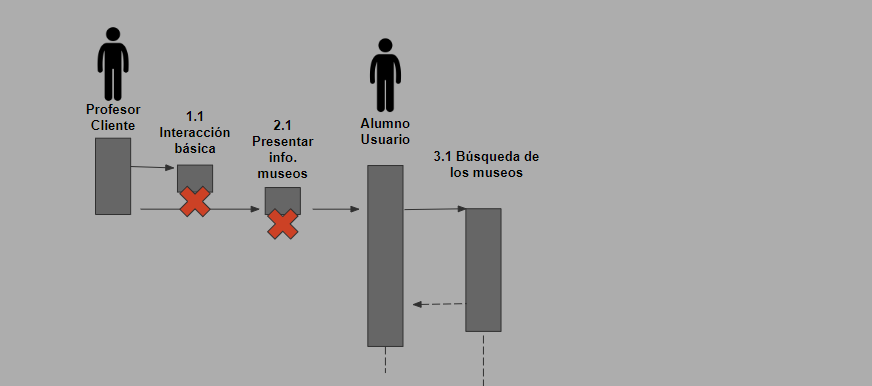
\includegraphics[width=15cm]{imgs/CasoUso_5_2.PNG}}
\caption{Caso-1}
\label{fig}
\end{figure}

\paragraph{Priorización}
{\textbf {Tipo:}}
Principal.

%%%%%%% CASO-6 %%%%%%%%%%%%%%%%
\newpage
\subsubsection{Uso por aficionado de los museos}

{\textbf {Resumen:}}
Un cliente habitual de los museos ve un folleto en la mesa principal de la entrada del museo, ve que hay una nueva App que permite ver el museo en su casa y que es interactivo, cuando vuelve a su casa, la descarga, imprime el código y empieza a descubrir cada una de las piezas del museo, fascinado con la aplicacion, comparte en redes sociales cada una de las piezas y el logro que obtuvo por completar el descubrimiento completo de las piezas de los museos regionales.

{\textbf {Actores:}}
Aficionado.

{\textbf {Propósito:}}
Evidenciar la conexión directa entre personas que frecuentas museos y la accesibilidad a la aplicación por parte de folletos dentro de los museos.

{\textbf {Referencias cruzadas:}}
R1.1, R1.2, R1.3, R1.4, R2.2, R2.3, R4.1, R4.2, R4.3, R4.4

\paragraph{Caso de Uso Esencial}

\begin{longtable}{|p{5cm}|p{8cm}|}
\hline 
Acción actores & Respuesta del sistema \\ 
\hline 
El usuario llega al lugar (museo) que contiene publicidad de la aplicación. & --- \\ 
\hline 
El usuario decide descargarla y utilizarla en su casa & --- \\ 
\hline
El usuario interactúa con la aplicación y descubre una pieza. & La aplicación da feedback de la pieza encontrada y muestra un botón para poder compartir directamente en redes sociales. \\ 
\hline
El usuario aprieta el botón para compartir en redes sociales. & Se despliega un panel con la información de la pieza para compartir y da la opción de que el usuario ingrese un mensaje personalizado. \\ 
\hline
El usuario escribe su mensaje y le da enviar. & El sistema  envía un formulario con la información pertinente a las redes sociales. \\ 
\hline

\end{longtable}

\paragraph{Diagrama de Caso de Uso}

\begin{figure}[H]
\centerline{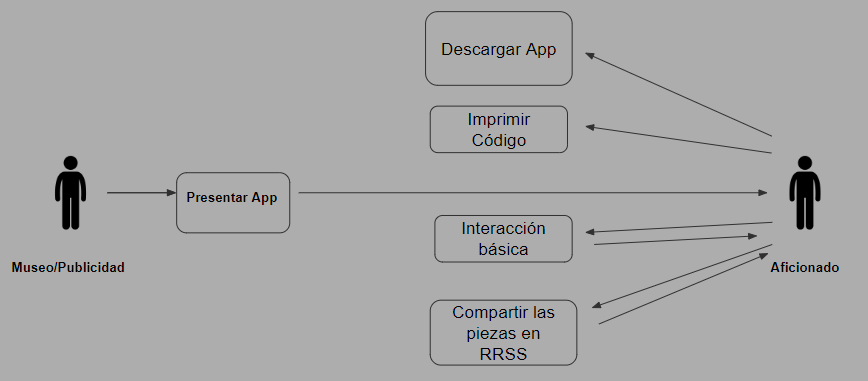
\includegraphics[width=15cm]{imgs/CasoUso_6.PNG}}
\caption{Diagrama Caso 6}
\label{fig_6_1}
\end{figure}

\paragraph{Modelo Conceptual}

\begin{figure}[H]
\centerline{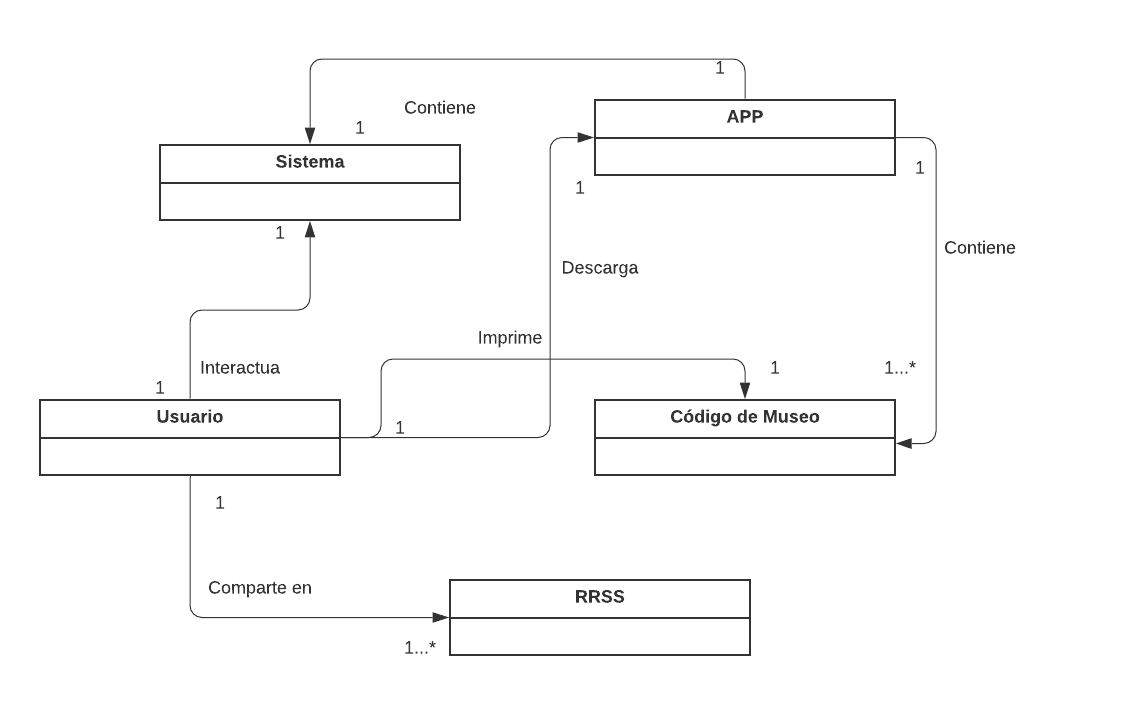
\includegraphics[width=15cm]{imgs/ModeloConceptualCaso_6_3.png}}
\caption{Modelo Conceptual Caso 6}
\label{fig_6_2}
\end{figure}

\paragraph{Diagrama de Secuencia o Colaboración}

\begin{figure}[H]
\centerline{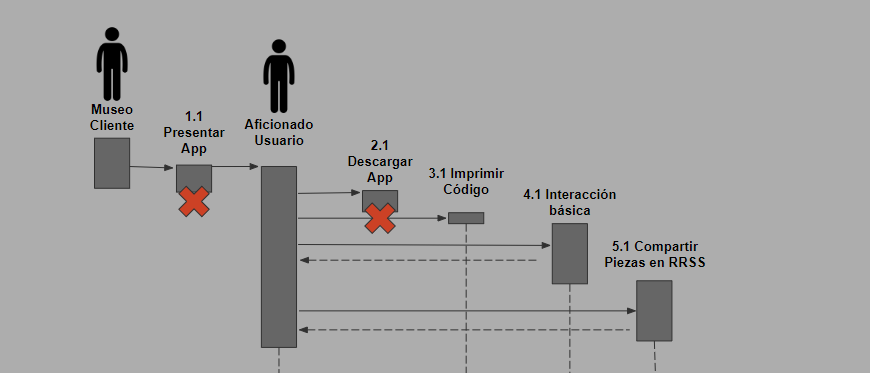
\includegraphics[width=15cm]{imgs/CasoUso_6_2.PNG}}
\caption{Diagrama de Secuencia Caso 6}
\label{fig_6_3}
\end{figure}

\paragraph{Priorización}
{\textbf {Tipo:}}
Principal.

%%%%%%% CASO-7 %%%%%%%%%%%%%%%%
\newpage
\subsubsection{Uso de la aplicacion por un estudiante y su familia}

{\textbf {Resumen:}}
Un alumno luego de llegar de la visita al museo regional, le muestra una aplicación nueva a su familia y les dice que si le pueden ayudar a encontrar las piezas que le faltan del museo que visito. Sus padres empiezan a jugar con él y encontrando cada uno de las piezas aprenden de su historia, además el alumno se divierte compartiendo con su familia con esta aplicación. El padre descubre luego de estar jugando un buen rato, que obtuvieron un logro, el abre el menú de logros y descubre que el juego cuenta con logros que han sido completados y otros que aún no se han desbloqueado, este le dice a su familia que sigan jugando para completar la mayoría.

{\textbf {Actores:}}
Alumno (hijo), Familia (padres y abuelos).

{\textbf {Propósito:}}
Demostrar el uso de la aplicación dentro de un entorno familiar y generar nuevos conexiones para enriquecer la comunicación familiar.

{\textbf {Referencias cruzadas:}}
R1.1, R1.2, R7.1, R7.2, R7.3, R7.4, R7.5, R7.6

\paragraph{Caso de Uso Esencial}

\begin{longtable}{|p{5cm}|p{8cm}|}
\hline 
Acción actores & Respuesta del sistema \\ 
\hline 
La familia ocupa la aplicación en su modo AR y descubre una pieza. & Se despliega un panel mencionando el descubrimiento y entrega un logro por encontrar todas las piezas de un ala del museo. \\ 
\hline 
El padre decide apretar el logro. & El sistema despliega un panel con los logros que ha encontrado hasta el momento. \\ 
\hline
--- & Enfocado en el que fue presionado. además se visualizan los logros que no han sido obtenidos. \\ 
\hline
El padre puede ver un información mínima sobre el logro y se dispone a sacarlos todos. & --- \\ 
\hline
\end{longtable}

\paragraph{Diagrama de Caso de Uso}

\begin{figure}[H]
\centerline{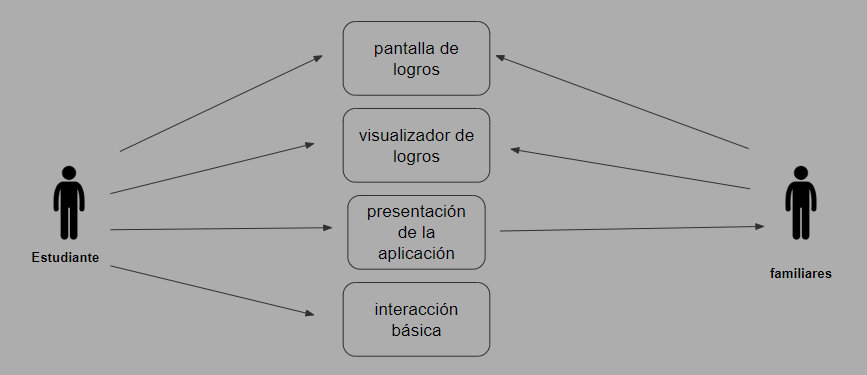
\includegraphics[width=15cm]{imgs/CasoUso_7.PNG}}
\caption{Caso-1}
\label{fig}
\end{figure}

\paragraph{Modelo Conceptual}

\begin{figure}[H]
\centerline{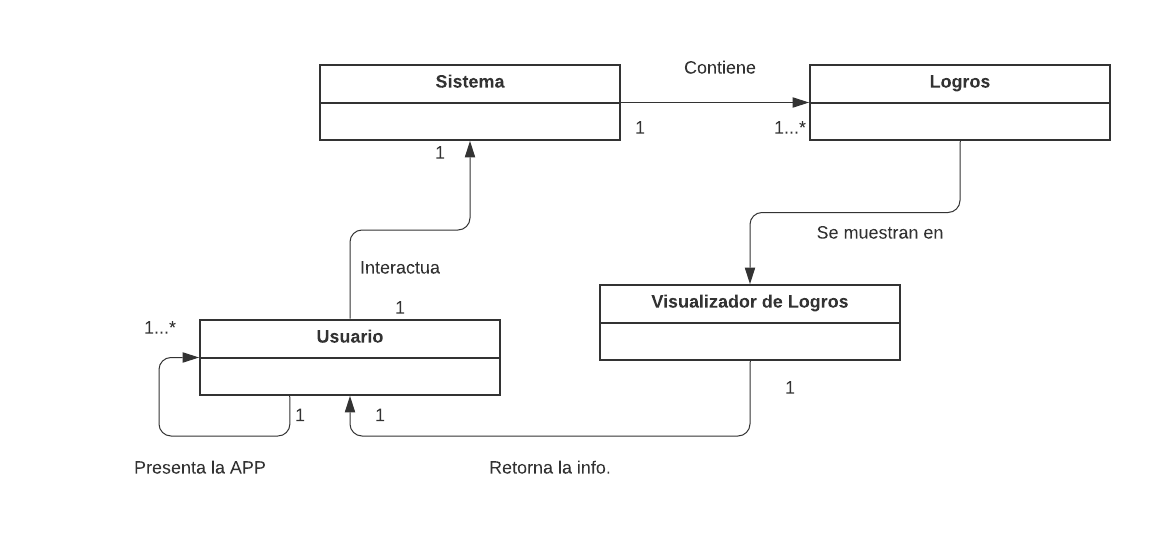
\includegraphics[width=15cm]{imgs/ModeloConceptualCaso_7_3.png}}
\caption{Caso-1}
\label{fig}
\end{figure}

\paragraph{Diagrama de Secuencia o Colaboración}

\begin{figure}[H]
\centerline{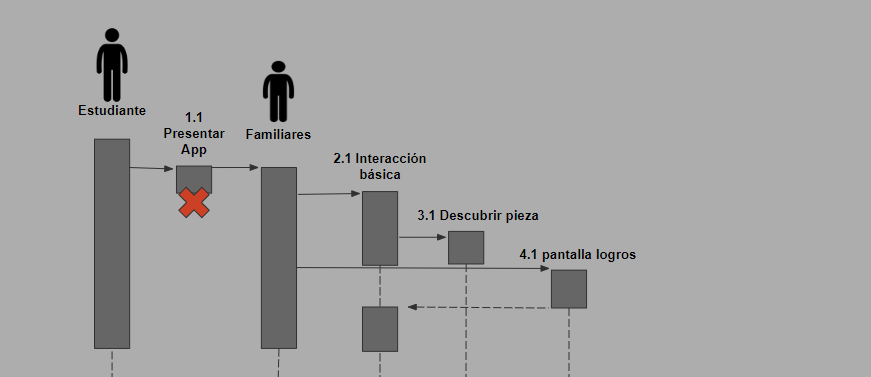
\includegraphics[width=15cm]{imgs/CasoUso_7_2.PNG}}
\caption{Caso-1}
\label{fig}
\end{figure}

\paragraph{Priorización}
{\textbf {Tipo:}}
Deseable.

%%%%%%% CASO-8 %%%%%%%%%%%%%%%%
\newpage
\subsubsection{Preparación de clase por parte de un profesor}

{\textbf {Resumen:}}
El nuevo director de UTP le dice al profesor de Historia de la existencia de una nueva App de Museos, el director quiere que el profesor haga uso de la aplicación en su clase. El profesor en su casa descarga la aplicación, imprime el código del museo que quiere mostrar en clases y empieza a buscar piezas, el profesor se da cuenta de que la app tiene logros, así que busca la manera de utilizar esos logros como décimas para la siguiente prueba del análisis de un museo histórico, en cuanto un alumno consiga un logro, se le asignará una décima. Ya en la clase el profesor empieza a mostrar la aplicación y enseña cómo obtener una pieza y muestra el tutorial completo de la manipulación de la pieza en 3d para ver los detalles de los modelos.


{\textbf {Actores:}}
Profesor, Director.

{\textbf {Propósito:}}
Demostrar el uso de la aplicación como herramienta de apoyo educativa dentro y fuera del aula.

{\textbf {Referencias cruzadas:}}
XXXX

\paragraph{Caso de Uso Esencial}

\begin{longtable}{|p{5cm}|p{8cm}|}
\hline 
Acción actores & Respuesta del sistema \\ 
\hline 
XXXX & XXXX \\ 
\hline 
\end{longtable}

\paragraph{Diagrama de Caso de Uso}

\begin{figure}[H]
\centerline{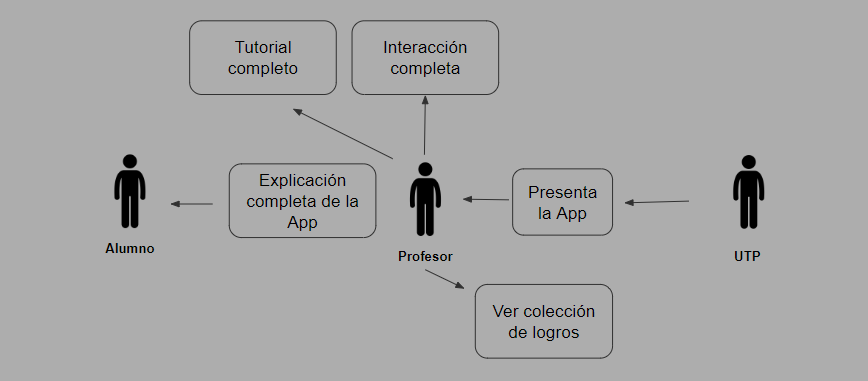
\includegraphics[width=15cm]{imgs/CasoUso_8.PNG}}
\caption{Caso-1}
\label{fig}
\end{figure}

\paragraph{Modelo Conceptual}

%\begin{figure}[H]
%\centerline{\includegraphics[width=15cm]{imgs/CasoUso_1_3.PNG}}
%\caption{Caso-1}
%\label{fig}
%\end{figure}

\paragraph{Diagrama de Secuencia o Colaboración}

\begin{figure}[H]
\centerline{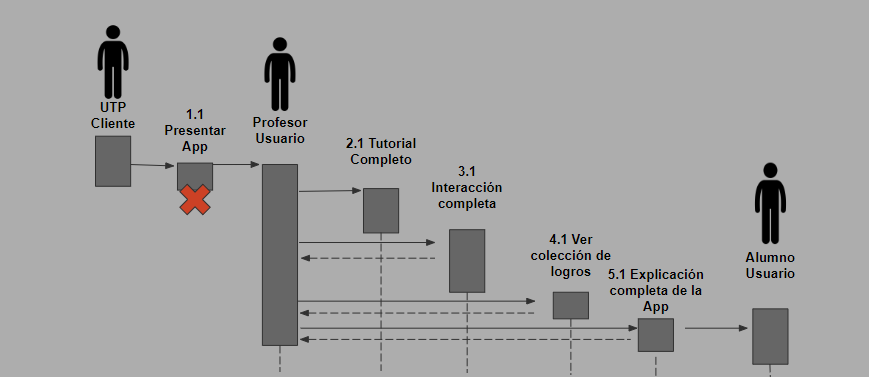
\includegraphics[width=15cm]{imgs/CasoUso_8_2.PNG}}
\caption{Caso-1}
\label{fig}
\end{figure}

\paragraph{Priorización}
{\textbf {Tipo:}}
Esencial.


\subsubsection{Contratos} %%apartado de contratos

\paragraph{Contrato 1} 
\begin{itemize}
\item Nombre: Escanear código QR
\item Responsabilidades: El sistema debe reconocer el código QR escaneado y obtener el museo referenciado a ese código QR, proyectando así el museo en la aplicación.
\item Tipo (concepto, clase de software, sistema): 
\item Referencias cruzadas: R 1.1, R 1.2
\item Caso de uso: 1.1 - 1.8
\item Notas: Nulo
\item Excepciones: Nulo
\item Salida: Nulo
\item Precondiciones: El código debe estar correctamente referenciado al museo en cuestión.
\item Poscondiciones: El museo debe ser el correspondiente al código QR y debe visualizarse en la aplicación.
\end{itemize}

\paragraph{Contrato 2} 
\begin{itemize}
\item Nombre: Obtener una pieza de museo y su info.
\item Responsabilidades: Obtener la pieza en cuestion, mostrar la información correspondiente y manejar la interacción con la pieza correctamente.
\item Tipo (concepto, clase de software, sistema): Sistema
\item Referencias cruzadas: R 2.1 - R 2.8, R 6.1 - R 6.8
\item Caso de uso: 1.1 - 1.8
\item Notas: Nulo
\item Excepciones: Nulo
\item Salida: Nulo
\item Precondiciones: La pieza debe estar correctamente referenciada a la información, a su vez debe mostrar el modelo correspondiente en el panel de información, en el menú de piezas y en el panel de interacción
\item Poscondiciones: El modelo debe ser interactuable, la información debe ser mostrada de manera legible y los botones de los paneles deben tener un funcionamiento establecido. 
\end{itemize}

\paragraph{Contrato 3} 
\begin{itemize}
\item Nombre: Obtener logro y su info.
\item Responsabilidades: Mostrar el logro obtenido y la información correspondiente.
\item Tipo (concepto, clase de software, sistema): Sistema
\item Referencias cruzadas: R 7.1 - R 7.6
\item Caso de uso: 1.6, 1.8
\item Notas: Nulo
\item Excepciones: Nulo
\item Salida: Nulo
\item Precondiciones:  El logro debe estar correctamente referenciada a la información, a su vez debe mostrar la información correspondiente a ese logro, 
\item Poscondiciones: En el menú de logros debe aparecen los logros completados y sin completar.
\end{itemize}

\paragraph{Contrato 4} 
\begin{itemize}
\item Nombre: Mostrar instrucciones
\item Responsabilidades: Las instrucciones deben mostrarse de manera correcta.
\item Tipo (concepto, clase de software, sistema): Sistema.
\item Referencias cruzadas: R 3.1 - R 3.4
\item Caso de uso: 1.1 - 1.8
\item Notas: Nulo
\item Excepciones: Nulo
\item Salida: Nulo
\item Precondiciones: Las instrucciones deben estar escritas correctamente y referenciadas al tutorial pertinente.
\item Poscondiciones: Las instrucciones deben ser mostradas de manera clara.
\end{itemize}

\subsection{Modelo de Dominio}
Un modelo de dominio en la resolución de problemas e ingeniería de software, es un modelo conceptual de todos los temas relacionados con un problema específico. Dentro de esta sección se analizarán las entidades reconocidas en los casos de uso para dar paso a la creación del Modelo de Dominio.

\subsubsection{Entidades Reconocidas}
Las entidades que fueron reconocidas en base al análisis de los casos de uso son:

\begin{itemize}
\item Pieza
\item Museo
\item Logro/Trofeo
\item Usuario
\item Menú
\item Colección
\item Visualizador
\item Tutorial
\item Sistema
\end{itemize}


\subsubsection{Modelo de Dominio}
En base a las entidades se realizo la asociación entre cada una y se genero el modelo de dominio.

\begin{figure}[H]
\centerline{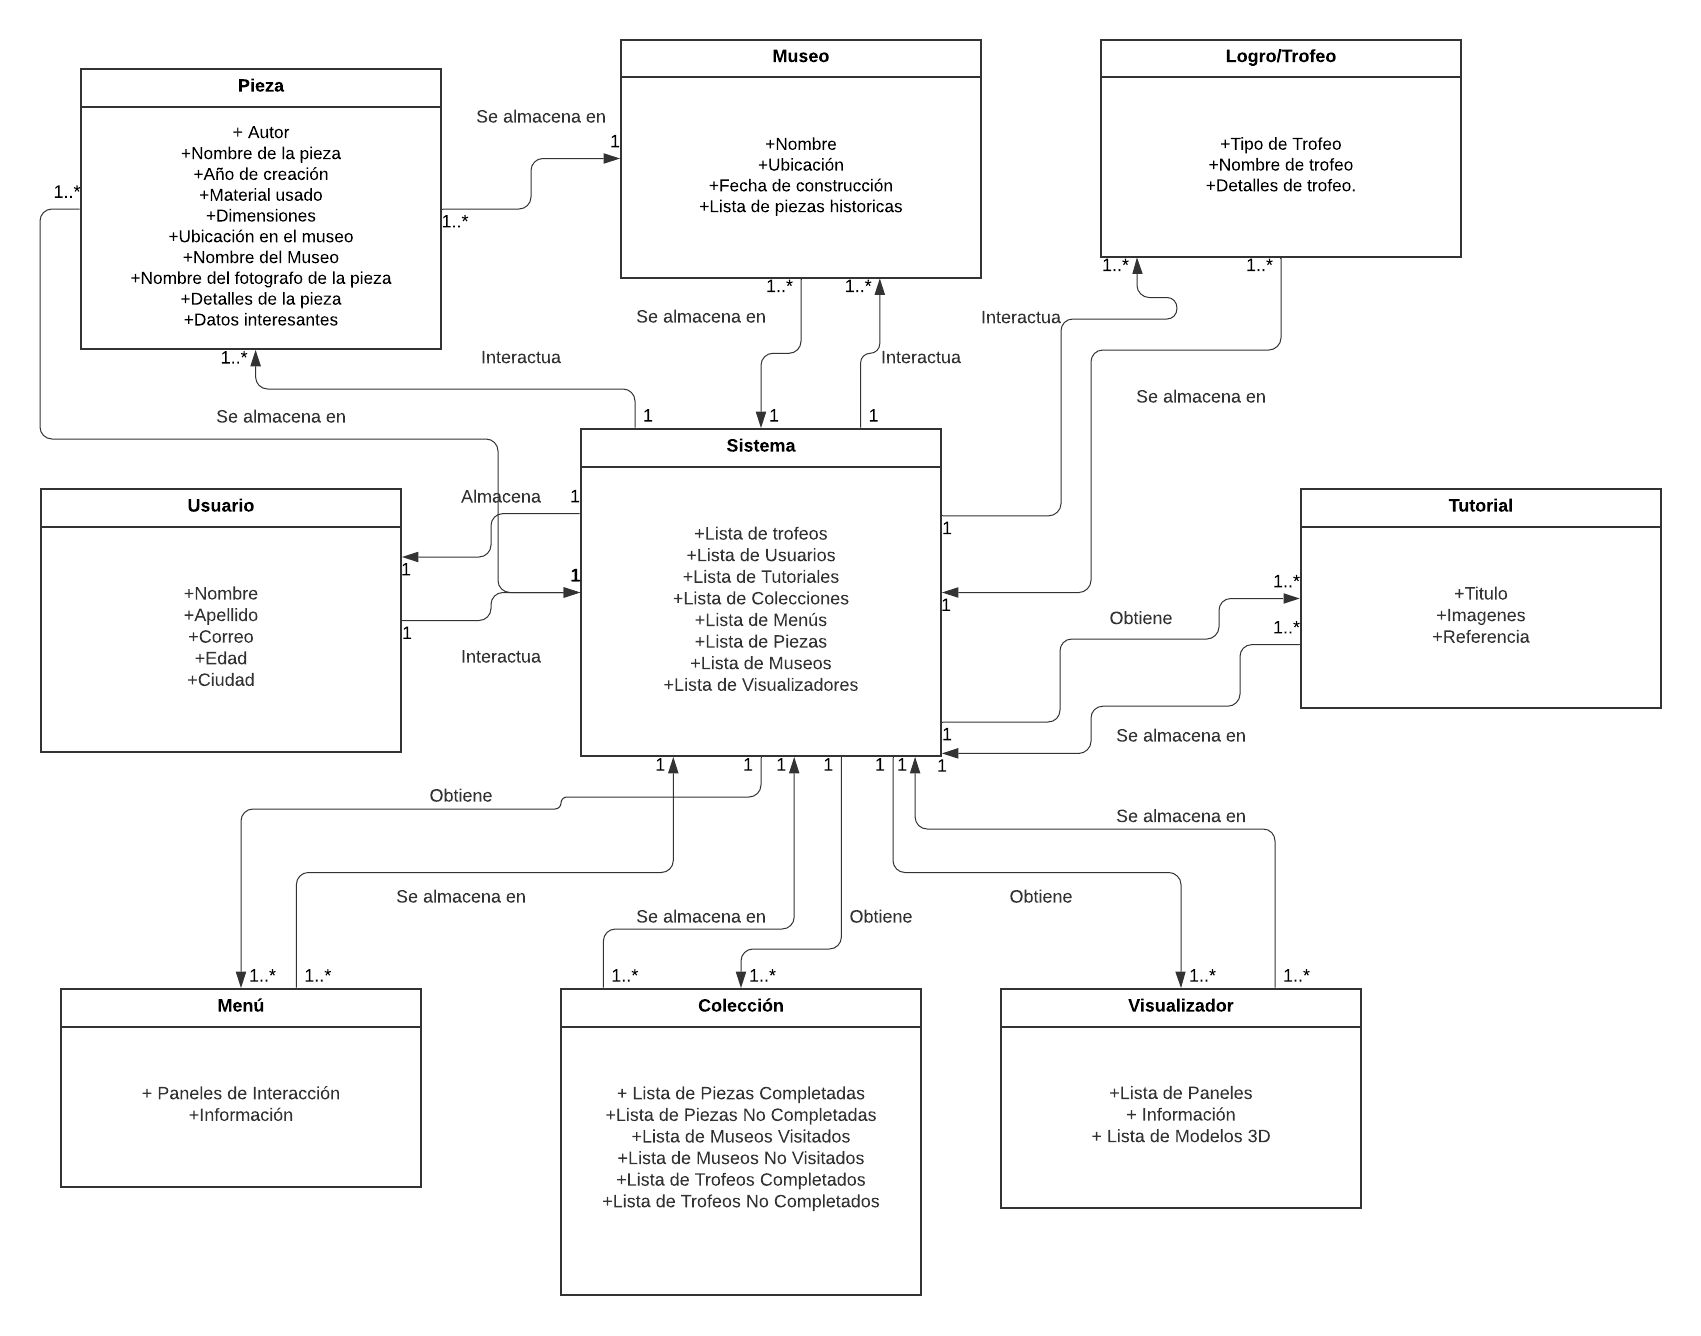
\includegraphics[width=15cm]{imgs/ModeloDeDominio.png}}
\caption{Modelo De Dominio}
\label{ModeloDom}
\end{figure}

\subsubsection{Matriz de Rastreabilidad}
\begin{longtable}{|c|p{1.3cm}|p{1.3cm}|p{1.3cm}|p{1.3cm}|p{1.3cm}|p{1.3cm}|p{1.3cm}|p{1.3cm}|}
\hline 
 & CU 1.1 & CU 1.2 & CU 1.3 & CU 1.4 & CU 1.5 & CU 1.6 & CU 1.7 & CU 1.8\\ 
\hline 
Pieza & X & X & X & X & X & X & X & X \\ 
\hline 
Museo &   &   &   &   & X & X &   &   \\ 
\hline
Logro/Trofeo &   &   &   &   &   &   & X & X \\ 
\hline
Usuario & X & X & X & X & X & X & X & X \\ 
\hline
Menú &   &   &   & X & X &   &   & \\ 
\hline
Visualizador &   &   & X &  &  	 &   & X & \\ 
\hline
Tutorial  &   & X &   &   &   &   &   & X \\ 
\hline
Colección &  &   &   &   &   &   &   & X \\ 
\hline
Sistema & X & X & X & X & X & X & X & X \\ 
\hline
\caption{Tabla de Matriz de Rastreabilidad}
\label{tab29}\\
\end{longtable}